\chapter{Theoretical Background}

\label{Chapter-Theoretical-Background}

The theoretical background of Machine Learning and Convolutional Neural Networks is being described below.

\section{Machine Learning}

Machine Learning, the name of which was first proposed in 1959 by Arthur Samuel \cite{Some-Studies-in-Machine-Learning-Using-the-Game-of-Checkers}, is a subset of Artificial Intelligence and a Computer Science (CS) field that studies algorithms and statistical models capable of performing specific tasks, such as prediction or decision making, without being explicitly programmed. Instead, sample data are used, also known as "training data", for the machine to "learn" to distinguish useful patterns on the input data capable of creating the needed output, e.g., decision or prediction. There are numerous approaches \cite{Machine-learning-Wikipedia} on the learning algorithms types, as well as on the model types used to get trained.

Such algorithm types, at the time of writing, include, but are not limited to:
\begin{itemize}
	\item \textbf{Supervised Learning:} Algorithms that learn by using "labeled" sample data, data that contain both the inputs and their desired outputs to be used for classification and regression.
	\item \textbf{Unsupervised Learning:} In contrast with the Supervised Learning, unlabeled sample data are used to discover structures that could group or cluster them.
	\item \textbf{Reinforcement Learning:} Algorithms responsible for taking actions in an environment, often also described as software agents, to maximize a specific metric, many of which use dynamic programming techniques.
	\item \textbf{Feature Learning:} Algorithms that by combining or even discarding features from the input samples, try to create a new, more useful set of features. One of the most popular algorithms of this category is Principal Components Analysis (PCA).
	\item \textbf{Anomaly Detection:} Algorithms that try to identify outlier samples, which are characterized by their significant difference compared to the majority of the data used. Such algorithms are often used in noise reduction, data mining, and even security and defense systems.
	\item \textbf{Association Rule Learning:} Algorithms that aim to discover strong relationships between features.
\end{itemize}

Such model types, at the time of writing, include, but are not limited to:
\begin{itemize}
	\item \textbf{Artificial Neural Networks (ANN):} Also known as Connectionist Systems, imitate the biological brain's neural networks.
	\item \textbf{Decision Trees:} Used to make assumptions about the input items' target value (the decision tree's leaves) via its observations (the decision tree's branches). When the target takes continuous values, the Decision Tree is called a Regression Tree.
	\item \textbf{Support Vector Machines (SVM):} Used for classification and regression, most\-ly famous as non-probabilistic, binary, linear classifiers. They can also be used for non-linear classification using the kernel trick.
	\item \textbf{Bayesian Networks:} Represented as directed acyclic graphs, they can include probabilistic relationships.
\end{itemize}

Nowadays, most industries have already used Machine Learning in some sort, indicating the significance and variety of its capabilities. It is estimated \cite{Machine-Learning-Applications} that by the year 2021, A.I. and M.L. spending will reach 57.6 Billion USD. Its applications include but are not limited to \cite{Top-Machine-Learning-Applications-in-2019} \cite{Roundup-Of-Machine-Learning-Forecasts-And-Market-Estimates}, web page ranking, image recognition, email filtering and spam detection, database mining, handwriting recognition, speech recognition, natural language processing, computer vision, image / video / text / speech generation, personalized marketing, travelling, dynamic pricing, healthcare, facial and fingerprint recognition and intrusion detection.

\section{Artificial Neural Network}

It is widely accepted that the brain's greatest ability is pattern recognition, which is used to combine "data" from the organism's senses in a way to better understand its environment. Artificial Neural Networks (ANN), a highly popular sub-field of Machine Learning, try to imitate the brain's structure to solve such problems, a structure that has been developing and proving its capabilities for thousands of years.

While ANNs are inspired by the biological neural networks, they are not identical. A neural network is a collection of connected neurons, through which electrical signals from sensor organs or other neurons are passed and processed. A biological neuron is comprised of four main parts; Dendrites, Cell body, Axon and Synaptic terminals (Figure \ref{fig:Standard-structure-of-a-biological-neuron}). A Dendrite and its Dendritic branches are used as the neuron's input, where sensors or other neurons get connected. A neuron can have multiple Dendrites. The neuron's cell body collects all the input signals and applies an "activation" function to create the output signal. Afterwards, the output signal is transported through the Axon and then distributed to the next neurons through the Synaptic terminals. The Synaptic terminals to Dendrites connections are called Synapses.

\begin{figure} [h]
	\centering
	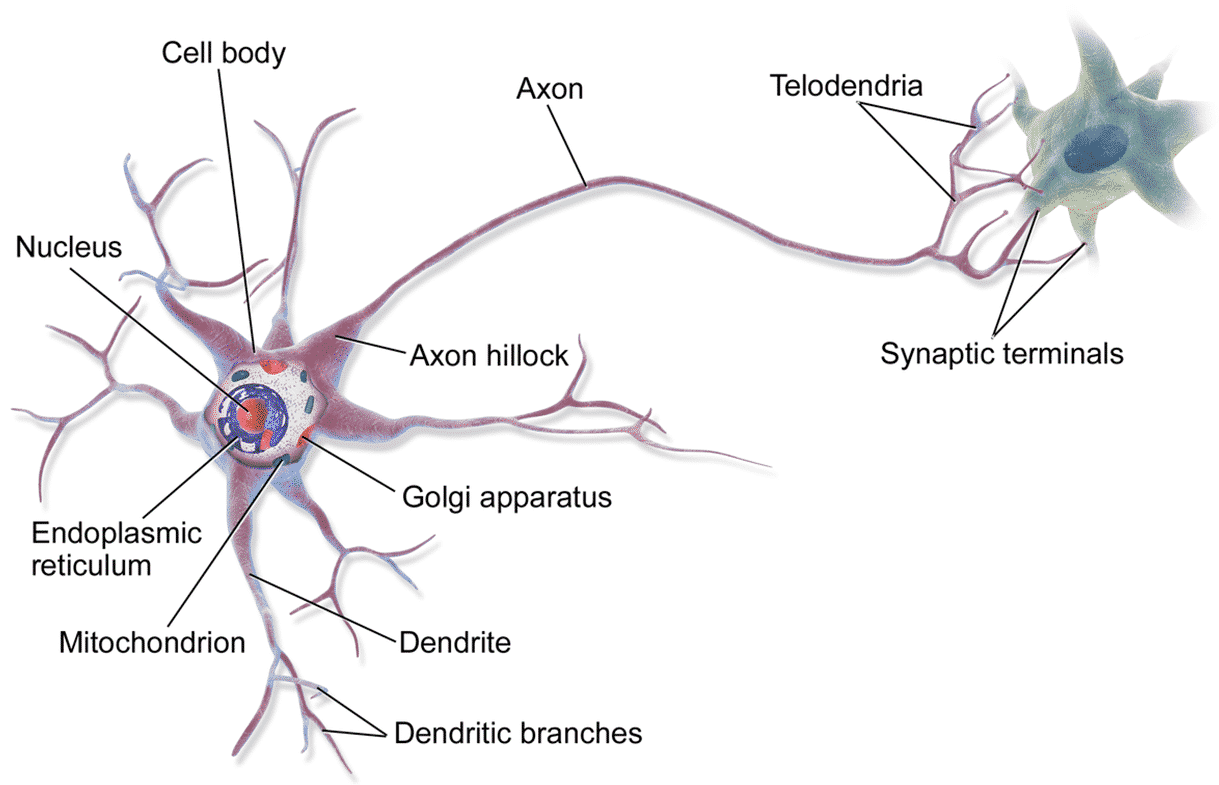
\includegraphics[width=\textwidth]{Images/Biological-Neuron.png}
	\decoRule
	\caption[Standard structure of a biological neuron]{Standard structure of a biological neuron: \href{https://nurseslabs.com/nervous-system/}{URL}}
	\label{fig:Standard-structure-of-a-biological-neuron}
\end{figure}

Similarly to the biological neural networks, an ANN can be represented as a graph, whose vertices represent the biological neurons' cell bodies and its edges the biological synapses. The electrical signal used in biological neurons is represented as a real number and their outputs are calculated by some non-linear function of the inputs' weighted sum. Each edge typically has a weight set during the training process, which amplifies or weakens the edge's signal.

% Todo: Add Basic components, e.g. neurons, activations, etc
% Todo: Explain what is a DNN
% Todo: Add NN architectures types, e.g. CNN, RNN, LSTM, etc

\section{Convolutional Neural Network}
\section{Structure of Convolutional Neural Network}
\subsection{Convolution Layer}
\subsection{Pooling}
\subsection{Activation Function}
\section{Typical Architecture of AlexNet}
